\documentclass[a4paper]{article}
\usepackage{amsmath,amssymb,caption,enumitem,float,geometry,graphicx,indentfirst,minted,parskip,tabularx,xcolor,verbatim}
\usepackage{booktabs}
\usepackage[utf8]{inputenc}
\usepackage[english]{babel}
\usepackage[backend=bibtex]{biblatex}
\addbibresource{Project.bib}
\captionsetup[figure]{labelsep=period}
\definecolor{bg}{rgb}{0.95,0.95,0.95}
\geometry{left=3.5cm,right=3.5cm,top=3.3cm,bottom=3.3cm}
\setlength{\parindent}{2em}
\usemintedstyle{emacs}
\begin{document}
\begin{titlepage}
    \vspace*{0.25cm}
    \noindent\rule[0.25\baselineskip]{\textwidth}{1pt}
    \begin{center}
        \huge{\textsc{UM--SJTU Joint Institute}}\vspace{0.3em}\\
        \huge{\textbf{Advanced Embedded System}}\vspace{0.3em}\\
        \Large{\textbf{(ECE4730J)}}
        \noindent\rule[0.25\baselineskip]{\textwidth}{1pt}
    \end{center}
    \begin{center}
        \vspace{5cm}
        \Large{\textsc{Project Proposal}}\vspace{0.5em}\\
        \Large{\textbf{ELMA: Encrypted Offloading for Embedded NLP Applications}}\vspace{1em}\\
        \Large{\textbf{Group 3}}\\
    \end{center}
    \vfill
    \large
    \begin{tabular}{ll}
        Name: Yihua Liu \hspace*{2em}&ID: 518021910998\hspace*{2em}\\
        Name: Shuocheng Chen \hspace*{2em}&ID: 517021911139\hspace*{2em}\\
        Name: Yiming Ju \hspace*{2em}&ID: 518370910059\hspace*{2em}\\
        \\
        Date: \today
    \end{tabular}
\end{titlepage}
\tableofcontents
\newpage
\section{Introduction}
NLP is short for Natural Language Processing, which focuses on the theories and methods of effective communication between human and computer in the field of natural language. It has developed for decades and has a wide use in our daily life, including text classification, auto correct, machine translation, speech recognition and so on. 

The applications of NLP are often user-oriented, which means it should take both portability and performance into consideration. To achieve a great performance, the data is often processed in the cloud because of its large computation. However, with an increasing number of smart devices, the data size also has an explosive growth and a tremendous scale of data is uploaded to cloud to perform analytics and predictions. Under this situation, there are some problems with such a terminal-to-cloud connection. Since the bandwidth is fixed, the network will be blocked if too much users attempt to connect at the same time. Thus the computation performance will be largely influenced. There may exist large latency and energy consumption during the data processing.

To cope with the cons of cloud computation, the concept of computation offloading is proposed. It offloads part of cloud computation to the terminal device. In this way, it not only helps solve the problem of cloud congestion but also accelerates computation and lower the latency through reducing data exchange with the cloud. Meanwhile, since the critical data can only be processed and stored locally, the security of individual private information can be guaranteed. 

Considering the size and performance of embedded devices, full offloading may lead to an opposite effect since the devices may take a long time to deal with the whole data processing locally.
Instead, partial offloading not only eases the pressure of computation in the cloud but also takes full advantage of local computation resources.

Our project will be focused on one of the applications of NLP, question answering. Namely, AI can automatically answer questions posed by humans, such as Siri and Google agent. Different from the traditional NLP models, a new language representation model called BERT is introduced in recent years, which stands for Bidirectional Encoder Representations from Transformers. It's a pre-trained model and can be fine-tuned with just one additional output layer to create state-of-the-art models of a wide range of tasks without substantial task-specific architecture modifications (BERT: Pre-training of Deep Bidirectional Transformers for Language Understanding). 

In this proposal, a short introduction and related works will be given in chapter 1 and 2. We will show our concept design and discuss some details in chapter 3. Then we will display our current progress and project plan in chapter 4.




\section{Related Work}
In the field of Natural Language Processing (NLP) and computation Offloading for embedded systems, there are several high-performance optimized neural network models and offloading methods from different perspectives.
\subsection{BERT: Bidirectional Encoder Representations from Transformers}
The Bidirectional Encoder Representations from Transformers (BERT) \cite{devlin2019bert} divides the NLP model into two steps: pre-training and fine-tuning. The transformer encoder is with Gaussian Error Linear Units (GELU) nonlinearities. BERT uses a Masked Language Model (MLM) for language model pre-training and a Next Sentence Prediction (NSP) task for text-pair representation pre-training. For fine-tuning, take question answering applications as an example, BERT takes question-passage pairs as input and feeds token and \textsf{[CLS]} representations to output layers.
\subsection{ALBERT: A Lite BERT}
ALBERT \cite{lan2020albert} does three significant improvements on traditional BERT model: factorized embedded parameterization, cross-layer parameter sharing, and inter-sentence coherence loss (sentence-order prediction (SOP) loss). ALBERT achieves better performance than BERT given larger configurations and fewer parameters. There are different methods to do cross-layer parameter sharing. ALBERT shares all parameters across layers by default, but parameters to share can be customized, such as feed-forward network (FFN) only or attention parameters only.
\subsection{EdgeBERT}
EdgeBERT is a hardware/software (more specifically, hardware/algorithm) co-design for multi-task NLP whose purpose is to reduce energy consumption as much as possible while achieving improvements of accuracy and speed \cite{tambe2021edgebert}. EdgeBERT proposes several main improvents, including entropy-based early exit (EE) and dynamic voltage-frequency scaling (DVFS). Our work is inspired by the strategies that EdgeBERT adopts to save energy, which is very important for embedded systems.
\section{Concept Design}
\begin{figure}[H]
    \centering
    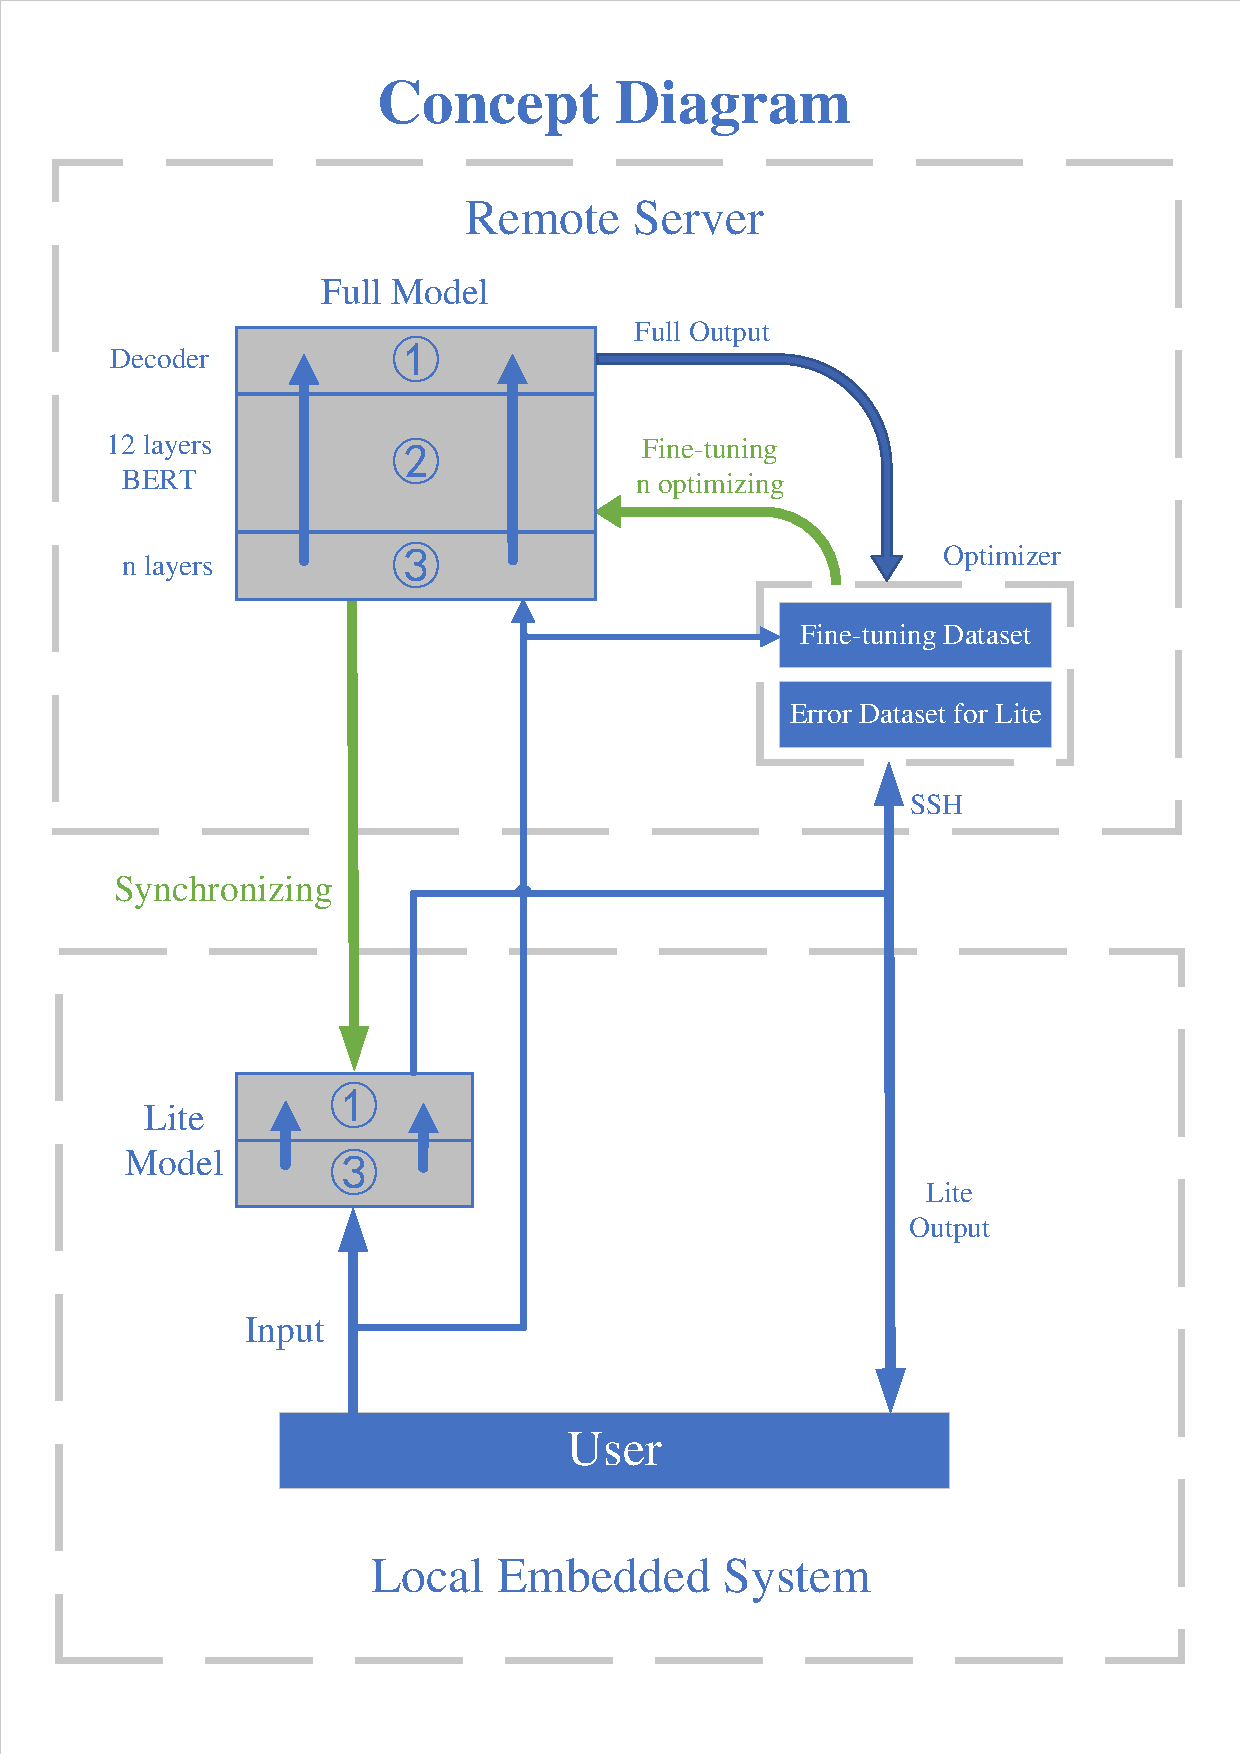
\includegraphics[width=1\textwidth]{Concept_Design.pdf}
    \caption{The diagram of the concept design.}
\end{figure}

\subsection{Transfer Learning}
Transfer learning is a research problem focusing on storing knowledge and applying it to a different but related task, which is to say, it aims to adapt an existing model to be endow with a different but related function that solves a different problem. There are two generally adopted approaches for tranfer learning, **feature extraction** and fine-tuning, between which the former one extracts the predicted features before the final classification from a pre-trained model and applies them to a new model, and the latter one retain the pre-trained model by further training the selected layers. 

Transfer learning separates the process of training from scratch (pre-training) and further adaptation and optimization, which enables computational redistribution to balance its resource consumption. Novel researches seek to utilize this feature to embedded devices, particularly after Covid-19 with the pattern recognition requirement for health monitoring devices, from which new inspirations of further application of transfer learning on embedded devices emerge.

\subsubsection{Feature Extraction}
Pre-trained deep learning models generate features corresponding to the input before the final output layer (usually a classifier or a decoder). The method of feature extraction seeks to utilize these features from pre-trained model as inputs to generate task-specific output, usually by training a customized classifier on a small specified dataset.

\subsubsection{Fine-tuning}
\begin{figure}[H]
    \centering
    \includegraphics[width=1\textwidth]{fine tune.png}
    \caption{Fine-tuning \cite{devlin2019bert}.}
\end{figure}
Fine-tuning re-trains selected layers of the pre-trained model while freezing other layers' parameters. An overall re-training would essentially cost extensive computation resources and could probably lead to disastrous forgetting, which promotes the problem and related research on fine-tuning methodologies. Nevertheless, fine-tuning is expected to perform better than feature extraction towards abundant tasks.

\subsection{NLP}
\subsubsection{Attention Mechanism and Transformer}
Attention mechanism is to generate an attention vector based on the input by certain algorithms that would be retained towards the decoding process. This is often done by passing a weighted sum of all encoder hidden states, which would provide extra information about the importance and connections of input words for the decoder.

Transformer is a rather novel architecture generally adopted for state-of-the-art NLP models, which is composed of a basic encoder-decoder structure with multi-head attention layers where the encoder compiles the input positional vectors (sequences) to certain vectors, and the decoder takes both the previous output and the encoder output to generate output probabilities, which can be further interpreted for task-completion.

\subsubsection{BERT}
Bidirectional Encoder Representations from Transformers (BERT) is a novel pre-trained model which is inspired by the encoder structure of transformers with a semi-original masked lanugage model which allows the predictions of masked tokens based on both directions of a single sequence. Its pre-trained nature allows the application of transfer learning approach to adapt it to different tasks, while its advanced architecture makes it applicable for many NLP tasks.

\section{Preliminary Project Timeline \& Current Progress}
The project is mainly divided into three parts, including preparation stage, function realization and presentation \& report part.

During the preparation stage, we are to do some literature review and purchase the related devices. Then by the end of the third week of October, we should have a detailed conceptual design.

For the part of function realization, we divide the implementation of all functions into three steps. In preliminary stage, our main task is to achieve the function of question answering on PC. Then we will add encryption algorithm to the model. After implementation, the work on the computer will be migrated to embedded devices. 

Our current progress has been shown in the gantt chart. We have already done a preliminary conceptual design and some literature review related to the BERT model. Then our next step is to transfer these models to the field of question answering and compare their performance so that we can appropriately choose a simple model for embedded devices and a complicated one for remote server.
\begin{figure}[H]
    \centering
    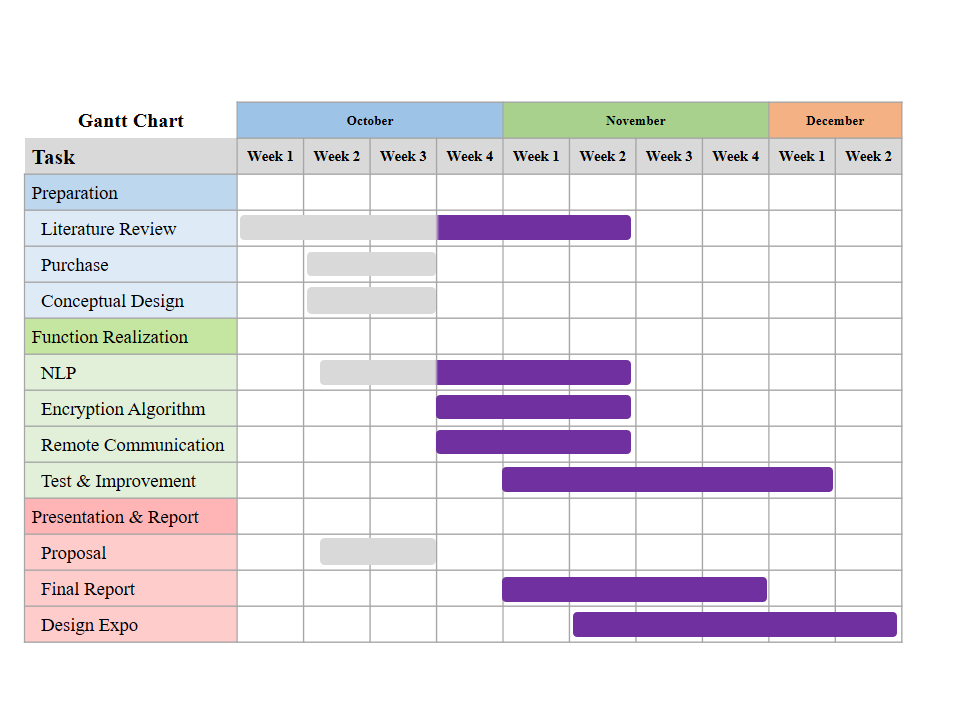
\includegraphics[width=1\textwidth]{Gantt Chart.png}
    \caption{Gantt chart of preliminary project timeline.}
\end{figure}
\printbibliography
\end{document}
